This chapter explains how to set up SITL ArduPilot Simulator in a virtual machine environment on Windows following the instructions the Ardupilot Dev Team tutorial. The tutorial was tested on Windows 10 with Oracle VM VirtualBox 5.2.12 and Ubuntu 16.04.
%http://ardupilot.org/dev/docs/setting-up-sitl-on-linux.html

Software In The Loop simulator allows to run ArduPilot code without any hardware. So SITL simulation is ideal to test new featues and changes in the code during development.

\section{Downloading the ArduPilot Code} \label{downloading_the_code}
%http://ardupilot.org/dev/docs/setting-up-sitl-on-linux.html
The ArduPilot project uses git for source code management and GitHub for source code hosting. To install git use the commands in the terminal:  %http://ardupilot.org/dev/docs/where-to-get-the-code.html#where-to-get-the-code

\begin{verbatim}
sudo apt-get update
sudo apt-get install git
\end{verbatim}

Now you have to get a copy of the ardupilot git repository. Open the terminal and run:
\begin{verbatim}
git clone git://github.com/ArduPilot/ardupilot.git
cd ardupilot
git submodule update --init --recursive
\end{verbatim}

Install required packages using the script \textit{install-prereqs-ubuntu.sh}  located in \textit{ardupilot/Tools/scripts}. Go to the directory you cloned ardupilot into and use the following command line. It can take a while depending on your internet connexion. Don't forget to accept the changes when asked.
\begin{verbatim}
cd ardupilot/Tools/scripts/install-prereqs-ubuntu.sh
\end{verbatim}

Now you have to add the following lines to the end of your \textit{.bashrc} file in your home directory. Notice the . on the start of that filename. Also, this is a hidden file, so if you’re using a file manager, make sure to turn on “show hidden files”.

\begin{verbatim} 
export PATH=$PATH:$HOME/ardupilot/Tools/autotest
export PATH=/usr/lib/ccache:$PATH
\end{verbatim}

Save the \textit{.bashrc} file and open the terminal. Then reload your PATH by using the “dot” command in a terminal:

\begin{verbatim} 
. ~/.bashrc
\end{verbatim}
If you don't change the  \textit{.bashrc} file you will not be able to use \textit{sim\_vehicle.py} as described in the next section.

\section{How to start SITL simulator}
In the terminal, go to the directory of the vehicle you want to make a simulation with. For example, for the multicopter code use the command line:
\begin{verbatim}
cd ardupilot/ArduCopter
\end{verbatim}

Then start the simulator using \textit{sim\_vehicle.py}. The first time you run it you should use the -w option to wipe the virtual EEPROM and load the right default parameters for your vehicle.
\begin{verbatim}
sim_vehicle.py -w
\end{verbatim}

After the default parameters are loaded you can start the simulator normally. First kill the sim\_vehicle.py you are running using Ctrl-C. Then:
\begin{verbatim}
sim_vehicle.py --console --map
\end{verbatim}

\section{FlightGear 3D View}  \label{sec_flightgear_view}

It is possible to install FlightGear Flight Simulator to display a 3D simulation of the vehicle and its surroundings. To install FlightGear from terminal use next command line. It may take a few minutes to finish the download.

\begin{verbatim}
sudo apt-get install flightgear
\end{verbatim}

If you want to run the simulation including the FlightGear 3D view, you need to open a new terminal, go to the directory \textit{/ardupilot/Tools/autotest/} and open \textit{fg\_quad\_view.sh} (Copter). This will start FlightGear. The next steps show the procedure to run the simulation.

\begin{enumerate}
\item In a terminal use the command lines:
\begin{verbatim} 
cd ardupilot/Tools/autotest
./fg_quad_view.sh 
\end{verbatim}

\item In other terminal:
\begin{verbatim} 
cd ardupilot/Ardu
sim_vehicle.py -j4 -L KSFO --map --console
\end{verbatim}

\end{enumerate}

In the step 2, KSFO indicates the location where the simulation will take place. FlightGear will always start by loading scenery at KSFO (San Francisco International Airport) but will change to the selected scenery once SITL is started.
If the vehicle appear to be hovering in space (no scenery) then you don't have the files for that location, but you can download it after. 

\subsection{Adding a new location to FlightGear}
	
    New locations are hard-coded into a file. This section shows how to add a new location. We will call the location as KSFO\_PAPI, because it will be next to PAPI lights in a lane of KSFO.
    
    In the directory \textit{ardupilot/Tools/autotest} find the \textit{locations.txt} file. This file contains all the locations you can choose for simulation. Each line follows the sintaxe:

\begin{verbatim}
#NAME=latitude,longitude,absolute-altitude,heading
\end{verbatim}  

Then add to the file the next line. 
\begin{verbatim}
KSFO_PAPI = 37.6136, -122.357, 5.3, 297.9
\end{verbatim}  
When you run the simulation in KSFO\_PAPI location using the steps shown in section \ref{sec_flightgear_view}, FlightGear environment will be as in figure \ref{fig_papi_lights}.

\begin{figure}[ht!] 
\centering
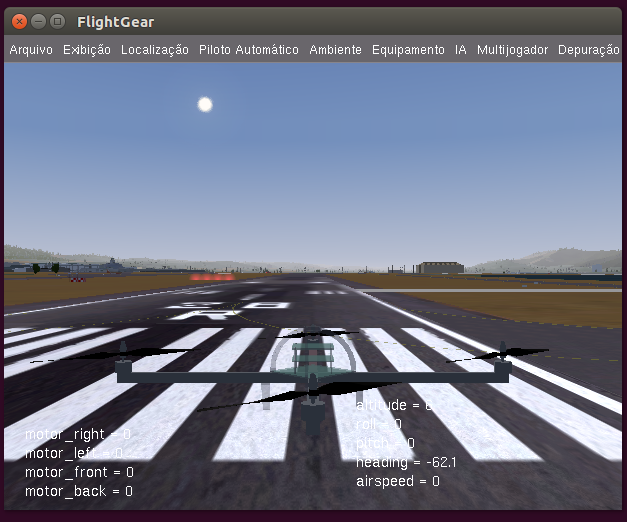
\includegraphics[width=1.0\textwidth]{Cap3/fig_papi_lights}
\caption{Image from FlightGear simulator running in SITL. Observe four red lights (PAPI) in the left of the lane. }
\label{fig_papi_lights}
\end{figure}




